\begin{quest}[Enumeratormachine]
	Definieer de enumeratormachine. Bewijs dat elke herkenbare taal kan ge\"enumereerd worden en dat elke taal die door een enumerator wordt ge\"enumereerd ook herkenbaar is. Kan elke beslisbare taal ge\"enumereerd worden? Bespreek in deze context de uitspraak ``de verzameling van Turing machines is een herkenbare taal''.
\end{quest}

De enumeratormachine is de machine zoals origineel voorgesteld door Alan Turing in 1936. Deze machine bezit deels de Turingmachine zoals we deze al kennen met enkele kleine aanpassingen. Zo heeft de machine ook een outputband, outputmarker en een enumeratortoestand $q_e$. De $\delta$ van de enumerator heeft als signatuur $$Q \times \Gamma \rightarrow Q \times \Gamma \times \Gamma_e \times \{L,R,S\}$$

Met $Q$ de huidige toestang en $\Gamma$ het te lezen symbool. Als output een nieuwe toestand $Q$ en $\Gamma$, samen met $\{L,R,S\}$. Het verschil met de Turingmachine die we eerder hebben gezien is $\Gamma_e$. Dit symbool zal bij overgang geschreven wordt op de outputband. Na het schrijven van $\Gamma_e$ verplaatst de outputmarker zich 1 plaats naar rechts. De output kan dan een string zijn, verschillende strings opgesplitst door een scheidingsteken  of zelfs een oneindige string... Eender hoe, het heeft zin om te spreken over de verzameling (eindige) outputstrings door de enumerator geproduceerd of ge\"enumereerd. Die verzameling is de taal door de enumerator bepaald of ge\"enumereerd. De enumerator mag daarbij dezelfde string meer dan eens op de outputband zetten.

\vspace{3mm}
\begin{figure}[h!]
  \centering
      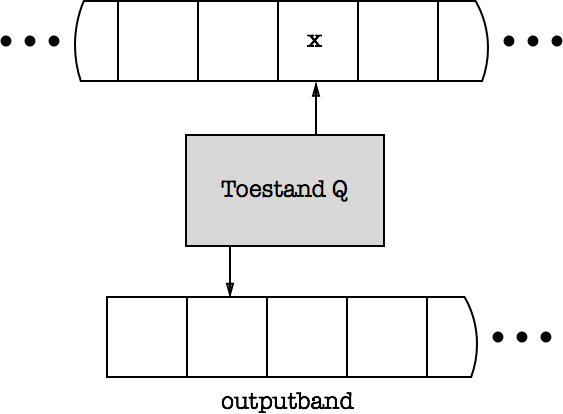
\includegraphics[width=0.5\textwidth]{./img/enumerator}
  \caption{Enumeratormachine.}
\end{figure}
\vspace{3mm}

\begin{theorem}
	De taal door een enumerator bepaald is herkenbaar en elke herkenbare taal wordt door een enumerator ge\"enumereerd. Beide stellingen zullen in aparte bewijzen worden bewezen.
\end{theorem}

\begin{proof}
	\textbf{Elke taal door een enumerator bepaald is herkenbaar.} Neem de Turingmachine $T$ voor de taal $L$, bepaald door een gegeven enumerator $E$. Laat $T$ nu $E$ als een subroutine gebruiken. $T$ neemt een string $s$ aan. Telkens $E$ in $q_e$ komt zal $T$ de laatst geproduceerde outputstring lezen op de outputband van $E$. Indien deze gelijk is aan de inputstring $s$, dan accepteert $T$ $s$. Indien dit niet zo is, gaat de enumerator doorrekenen\footnote{De enumerator kan dus oneindig blijven doorrekenen waardoor de taal door een enumerator bepaald herkenbaar en niet beslisbaar is.}.
\end{proof}

\begin{proof}
	\textbf{Elke herkenbare taal wordt ge\"enumereerd door een enumerator.} Neem de Turingmachine $T$ die de willekeurige taal $L$ herkent. Het is voldoende een enumerator $E$ te construeren die $L$ enumereert\footnote{Indien dit lukt is dit mogelijk voor elke $L$, aangezien $L$ willekeurig is.}. Om $E$ op te stellen, maken we gebruik van enkele hulpmachines.\\
	\begin{enumerate}
		\item Een machine $T_{gen}$ die voor een gegeven getal $n$ de eerste $n$ strings uit $\Sigma^*$ genereert\footnote{Namelijk $s_1,s_2, \dots ,s_n$.}. Deze $T_{gen}$ zal de strings op de band van $E$ plaatsen.
		\item $T_n$  zal op elk van de gegeven $n$ strings, $n$ stappen van $T$ uitvoeren. Het zal dus het aantal stappen van $T$ limiteren zodat deze niet in een oneindige lus kan gaan voor de strings die niet worden herkend. Waarom doen we dit? We willen eigenlijk alle strings overlopen\footnote{Die mogelijk zijn op het alfabet $\Sigma$.} en daar de aanvaardbare strings ($s \in L$) uit filteren. Deze behoren tot de herkenbare taal $L$. Hierdoor moeten we ook de strings nakijken die niet tot $L$ behoren. Deze kunnen er echter voor zorgen dat de $T$ in een oneindige lus gaat. Daarom limiteren we het aantal stappen zodat ook $E$ niet oneindig moet blijven wachten. Indien $T$ de string aanvaardt, plaatst $E$ de string op de outputband. Indien $T$ deze niet aanvaard of niet ge\"eindigd is in $\leq n$ stappen, dan zal $E$ de string niet schrijven.
		\item $T_{driver}$ zal een opeenvolging van getallen $n$ genereren om de voorgaande machines op te stellen en $T_{gen}$ en $T_n$ oproepen.\\
	\end{enumerate}
	Resultaat: Alle $s \in L$ zullen op de outputband worden gezet, maar toch zal de uitvoering van de oneindige lus gestopt worden zodat de enumerator zeker eindigt. Hiermee is het halting probleem voorkomen. Well done.
\end{proof}

Ten slotte moeten we vermelden dat elke taal die beslisbaar is kan ge\"enumereerd worden, aangezien elke beslisbare taal ook herkenbaar is. Uit het laatste bewijs zou ook duidelijk moeten zijn dat $A_{TM}$ een herkenbare taal is. We voeren het bewijs gewoon opnieuw uit, maar met $L = A_{TM}$. Dus in plaats van $T$ $n$ stappen te laten lopen over een inputstring, laten we nu $M$ $n$ stappen lopen over $s$ (uit $<M,s>$ $\in A_{TM}$).
